Betrachten Sie folgendes Klassendiagramm, welches leider ungültig ist:



\begin{centering}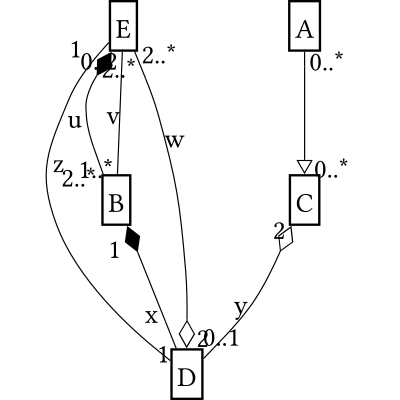
\includegraphics[min width=0.4\textwidth=0.6\textwidth,min height=0.4\textwidth=0.6\textwidth,keepaspectratio,max width=0.9\textwidth,max height=0.9\textwidth]{54/cdf0c034ae2b2d873c2c8affabc7eea3fa50026d3c82dac65b2adc16b689fafc6a01af83b04c596701db35357ce8aed00a3a92e08161.pdf}\end{centering}



Es enthält die folgenden Beziehungen zwischen Klassen:

\begin{enumerate}\item[ 1 ]{Komposition x}
\item[ 2 ]{Aggregation w}
\item[ 3 ]{Aggregation y}
\item[ 4 ]{Komposition u}
\item[ 5 ]{die Vererbung, bei der A von C erbt, bei der die Multiplizität 0..* neben A und 0..* neben C angegeben ist}
\item[ 6 ]{Assoziation z}
\item[ 7 ]{Assoziation v}
\end{enumerate}

Wählen Sie aus, was Sie für den einen Grund dafür halten, dass dieses Klassendiagramm ungültig ist, und nennen Sie alle Beziehungen, die definitiv zum Problem beitragen, d.h., deren Entfernung das Problem jeweils beheben würde.

Gründe, die hierfür zur Auswahl stehen, sind:

Das Klassendiagramm ...

\begin{enumerate}\item[ a ]{enthält mindestens zwei Nicht-Vererbungsbeziehungen zwischen denselben beiden Klassen, die in entgegengesetzte Richtungen zeigen.}
\item[ b ]{enthält mindestens ein Paar von Klassen, die sich gegenseitig beerben.}
\item[ c ]{enthält mindestens eine Selbstvererbung.}
\item[ d ]{enthält mindestens einen Vererbungszyklus.}
\item[ e ]{enthält mindestens eine nicht erlaubte Multiplizität am Ganzen einer Komposition.}
\item[ f ]{enthält mindestens eine Selbstbeziehung, die keine Vererbung ist.}
\item[ g ]{enthält mindestens eine nicht erlaubte Multiplizität an einer Vererbung.}
\item[ h ]{enthält mindestens einen Kompositionszyklus.}
\item[ i ]{enthält mindestens eine Mehrfachvererbung.}
\item[ j ]{enthält mindestens zwei Nicht-Vererbungsbeziehungen zwischen denselben beiden Klassen.}
\end{enumerate}

Bitte geben Sie Ihre Antwort an, indem Sie Folgendes angeben: einen Buchstaben für den Grund, der Ihrer Meinung nach der am spezifischsten ausgedrückte Grund dafür ist, dass dieses Klassendiagramm ungültig ist, und eine Auflistung von Zahlen für diejenigen Beziehungen, von deren individueller Präsenz das Problem abhängt. Zum Beispiel würde

\begin{verbatim}due-to:
- 3
- 4
reason: b
\end{verbatim}

bedeuten, dass das Klassendiagramm wegen Grund b ungültig ist und dass die 3. und 4. Beziehung (zusammen auftretend) das Problem erzeugen.



Bitte beachten Sie: Klassen werden hier vereinfacht dargestellt. 
 Das heißt, sie bestehen aus einer einfachen Box, die nur den Klassennamen enthält, aber keine Abschnitte für Attribute oder Methoden. 
 Trotzdem sollten Sie diese vereinfachten Klassendarstellungen als valide Klassen ansehen.

Bitte beachten Sie: Beim Bewegen über oder Klicken auf Kanten / Knoten bzw. ihre Beschriftungen werden die jeweils zusammengehörenden Komponenten hervorgehoben.

